%%%%% Dokumentenklasse mit verschiedenen Attributen
\documentclass[a4paper, bibtotocnumbered,liststotoc,12pt,abstracton]{scrartcl}

%%%%% Betriebssystemabh�ngige Eingabedekodierung
\usepackage[T1]{fontenc}
\usepackage[latin1]{inputenc} %% f�r Windows

%%% Python code
\usepackage{listings}             % Include the listings-package
\lstset{language=Python}          % Set your language (you can change the language for each code-block optionally)


%%%%% \usepackage[applemac]{inputenc} %% f�r Mac
\usepackage[ngerman, english]{babel}

%%%% Arial
%\usepackage{uarial}
%\renewcommand{\familydefault}{\sfdefault}
%\usepackage{blindtext}

%%%%% Zeilenabstand
\usepackage{setspace}
\onehalfspacing %anderthalbzeilig

%%%%% Mathematik und Symbole
\usepackage{amsmath}
\usepackage{amssymb}
\usepackage{amsthm}

%%%%% Seitenr�nder und Ausrichtung
\usepackage[paper=a4paper,left=30mm,right=25mm,top=25mm,bottom=35mm]{geometry} %define margins..
\geometry{a4paper} % hier auch m�glich 'letter' oder 'a5paper' ... etc.
\usepackage{lmodern}
\usepackage{verbatim}
\setkomafont{sectioning}{\rmfamily\bfseries\boldmath}
\usepackage[usenames,dvipsnames]{color}


%%%%% �berschriften
%\pagestyle{headings} %F�gt �berschrift �ber jeder Seite ein

\usepackage{overcite}

%%%%% Tabellen und Grafiken
\usepackage{booktabs}
\usepackage{tabularx}
\usepackage{array}
\usepackage{graphicx}
\usepackage{rotating}
\usepackage{xtab}
\usepackage{float}

%%%%% Sonstiges

%%%%% Umgebungen f�r S�tze, Propositionen,...
\newtheorem{hyp}{Hypothesis}
\newtheorem*{beweis}{Beweis}
\newtheorem{theorem}{Theorem}
\newtheorem{determinant}{Determinant}

%%%%%%%%%%%%%%%%%%%%%%%%%%%%%%%%%%%%%%%%%%%%%%%%%%%%%%%%%%%%%%%%%%%%%%%
%%%%% BEGIN DOCUMENT %%%%%%%%%%%%%%%%%%%%%%%%%%%%%%%%%%%%%%%%%%%%%%%%%%%%%%%
\begin{document}
\selectlanguage{english}

%%%%%%%%%%%%%%%%%%%%%%%%%%%%%%%%%%%%%%%%%%%%%%%%%%%%%%%%%%%%%%%%%%%%%%%
%% TITLE PAGE %%%%%%%%%%%%%%%%%%%%%%%%%%%%%%%%%%%%%%%%%%%%%%%%%%%%%%%%%%%%%%
\selectlanguage{ngerman}
\begin{titlepage}
\large{Timo Meiendresch}
 \vspace{\fill}
\begin{center}
\Huge{Recurrent Neural Networks for Time Series Forecasting}\\
\large{}
\end{center}
 \vspace{\fill}
\large{Capstone Project} \\
\large{Machine Learning Engineer Nanodegree (Udacity)}\\
\vspace{\fill}\\ Cologne 2019\\
%Cologne
\end{titlepage}
\selectlanguage{english}
%%%% Inhalts-, Abbildungs- und Tabellenverzeichnis
\tableofcontents %f�gt ein Inhaltsverzeichnis ein
%\listoffigures % f�gt ein Abbildungsverzeichnis ein 
%\listoftables % f�gt ein Tabellenverzeichnis ein %\newpage % Seitenumbruch %%%%%%%%%%%%%%%%%%%%%%%%%%%%% Hauptteil %%%%%%%%%%%%%%%%%%%%%%%%%%%%%%%
\newpage
\begin{abstract} 
The year is 2019 A.D. Quantitative research is entirely occupied by Machine Learning (ML). Well, not entirely... One small group of indomitable forecasters still holds out against the invaders. And life is not easy for the ML evangelists who garrison the fortified camps of quantitative research. 
\end{abstract}

\section{Introduction}
% Importance of time series forecasting
Time series forecasting is an essential tool in business, economics, and many other disciplines. The ability to accurately infer future variables given historic data is of huge value to decision makers. 

% Surge of ML methods 
In recent years, \textbf{Machine Learning (ML)} methods had huge success in many areas of quantitative research. Prominent examples include classification tasks, image processing, or text analysis. ML took many fields by storm and it seems that many quantitative discipline can benefit from giving in to the AI wave.

% Contrast to time series forecasting
And yet, ML methods are rarely considered in time series forecasting. Research within this field indicated an inferior performance compared to traditional methods. Moreover, those methods are often easier to implement, are computationally cheap, and better interpretable. Important examples include the \textbf{Autoregressive Integrated Moving-Average (ARIMA)} and the various \textbf{Exponential Smoothing (ES)} methods. 

% Notion
Until recently, a widely shared notion was that complex methods for time series forecasting generally were not performing better than traditional ones (e.g. Hyndman, 2019). Among others, Makridakis et al. (2018) noted that there is only very limited scientific evidence which suggests that artificial neural networks may be a useful tool for time series forecasting. 


\subsubsection*{Paradigm Shift}
But, advances in recent years start to challenge this perception. For example, the winner of the most recent version of the M4 time series forecasting competition (Makridakis et al., 2019) was an elaborate hybrid of a \textbf{recurrent neural network (RNN)} architecture with ES methods (Smyl, 2019). Measured on a diverse dataset of 100,000 univariate time series from six domains and frequencies, this method outperformed traditional ones, pure statistical combinations as well as ML-based combination methods. The results of the competition showed the potential of recurrent networks for time series forecasting, leading to a surge of algorithms in this area. It also showed that RNN could successfully be trained on highly diverse data. Commonly, RNN methods for time series foreasting are applied to a large set of homogeneous data.  

\subsubsection*{Local vs. global methods}
Moreover, the M4 competiton highlights an ongoing paradigm shift in the forecasting community. Traditional methods like ARIMA and ES are applied to individual series. These \textbf{local} methods estimate a number of parameters within a model space that is restricted by the respective structure of the model. Because these approaches rely on an explicit model structure they are referred to as \textbf{model-based} (Wang et al., 2019). Each time series is modeled and trained independently of other series in the data set. Hence, the individual model is independent of the total number of series in the as well as how similar these series are.

Also, with the emergence and availability of large sets of data, a new forecasting problem emerged. It is becoming increasingly necessary to implement large-scale forecasting systems that simultaneously predict many, often related, series. Examples include predictions of product sales in online retailers, household energy consumption, or web traffic. In contrast to local models, \textbf{global} methods enable the use of \textbf{cross-series learning}, i.e. during training process all available time series are used. This approach is supposed to yield a general representation of the entire data set. In theory, RNN-based methods should be able to learn across individual series and extract general patterns of the data as well as learn dependency relationships between the individual series which may improve forecasting accuracy. This may improve the forecast accuracy over local approaches.

There are various methods based on the idea of cross-series learning, in particular utilizing recurrent networks. The determinants of their performance is a relatively new question into which very little empirical research has so far been done. 

In theory, RNN should be able to work as a universal function approximator if it is only powerful enough. In practice however, the learnability of RNNs is limited. A typical problem is that they do not converge during training. They are considered to be difficult to train. This is an important factor for practitioner's as training a powerful network on such a huge amount of data is computationally expensive. 

For now, it seems that there are two key determinants that should be considered in the performance of the models: 

\begin{determinant}
Total number of individual time series in the underlying data set. How many series are in the dataset?
\end{determinant}

\begin{determinant}
Similarity of the individual time series in the data set. How diverse are the series?
\end{determinant}

This leads to two hypothetically important caveats regarding the dataset which influence the performance. The total number of time series in the dataset as well as how diverse the series are with respect to each other.

Often, these methods lack rigorous comparison with previous methods and known data sets. This capstone project investigates the performance of three RNN-based methods developed in the last three years, namely: 

\begin{itemize}
\item \textbf{Deep Autoregressive Recurrent Neural Networks (DeepAR)} - Wang et al. (2017)
\item \textbf{Deep State Space Models (DeepState)} - Rangapuram et al. (2018)
\item \textbf{Deep Factor Recurrent Neural Network Model (DF-RNN)} - Wange et al. (2019)
\end{itemize}

To evaluate these models I will apply them to the Hourly, Daily, Weekly and Monthly data of the M4 competition using the same measures of accuracy. Hence, a variety of benchmarks is available for comparison. 

% Heterogeneous data vs. Homogeneous data?
Note that these methods are designed to be applied to large sets of related data. In contrast, the M4 data set is a diverse dataset from many domains and frequencies.

To the best of my knowledge, no empirical investigation of these algorithms to the M4 benchmarks has been published yet. The primary contribution of this paper is to evaluate these algorithms on the well studied M4 data and compare the results to known benchmarks. 

The rest of the paper is organized as follows. I first discuss ... in Section ....

\section{Definition}
\subsection{Project Overview}
% High-level overview of the project
% Background information such as the problem domain
% Project origin
% related data sets or input data given
This project compares three RNN-based algorithms for time series forecasting to the well studied M4 data and its benchmarks, including modern and traditional methods. The datasets include the original M4 data for hourly, daily, weekly, and monthly frequencies. 

\subsection{Problem Statement}
% Clearly defines the problem
% Strategy for solving the problem
% Discussion of expected solution
Main goal of this paper is to evaluate the performance of three algorithms on the M4 data. The algorithms are DeepAR, DeepState, and DF-RNN. These results will be compared with traditionally widely used methods as well as state-of-the art methods that were part of the competition. The main goal is to assess their their competitiveness using default hyperparameters. 

\subsection{Metrics}
The performance of the methods is evaluated using the same two measures that were used in the M4 competition. Forecast measures are still a highly active area of research and there is no consensus on which one is considered to be the best one. Hence, two widely used \textbf{scale-independent errors} were used in the competition. Scale-independent means they are independent of the unit of the time series. Because the competition evaluates accuracy across highly diverse time series, scale-independent measures are required. The two measures are:
\begin{itemize}
\item \textbf{Symmetric mean absolute percentage error (sMAPE)}
\item \textbf{Mean absolute scaled error (MASE)}
\end{itemize}
The \textbf{sMAPE} belongs to the class of percentage errors which are unit-free. One drawback of the measure is that it is infinite/undefined if the target variable is zero for any $t$ in the period of interest, and is highly skewed towards extreme values if the target variable is close to zero. The measure is defined as 
\begin{align*}
sMAPE = \frac{1}{h} \sum_{t=1}^h \frac{2 \,|Y_t-\hat{Y}_t |}{|Y_t| + |\hat{Y}_t|}
\end{align*}
where $Y_t$ is the post-sample value, $\hat{Y}_t$ the estimated forecast, and $h$ the forecasting horizon.

Alternatively, Hyndman and Koehler (2006) propose the scaled error measure \textbf{MASE} when comparing forecast accuracy across series with different units. In this case the absolute error is scaled using the \textbf{Mean Absolute Error (MAE)} from a simple forecast method (either naive or seasonal naive method). The method is defined for seasonal data in the following way: 
\begin{align*}
MASE = \frac{1}{h} \, \frac{ \sum_{t=1}^h |Y_t - \hat{Y}_t| }{ \frac{1}{n-m} \sum_{t=m+1}^n |Y_t - Y_{t-m}|}
\end{align*}
where $m$ indicates the seasonality of the series. In case of non-seasonal data ($m=1$), $Y_t - Y_{t-m}$ simplifies to $Y_t - Y_{t-1}$ being the naive forecast error. The naive forecast predicts the next value to be equal to the last value $\hat{Y}_{t+1} = Y_t$. This yields the non-seasonal version of the MASE as 
\begin{align*}
MASE = \frac{1}{h} \, \frac{ \sum_{t=1}^h |Y_t - \hat{Y}_t| }{ \frac{1}{n-m} \sum_{t=m+1}^n |Y_t - Y_{t-m}|}
\end{align*}
In addition to measuring point forecast accuracy using MASE and sMAPE, prediction interval accuracy has also been introduced in the competition for the first time. For this, the \textbf{Mean Scaled Interval Score (MSIS)} has been used as accuracy measure. Furthermore, other widely used measures for evaluating forecast accuracy include the normalized sum of quantile losses for quantiles $p \in {0.5, 0.9}$. These were the preferred measures in some of the mentioned papers which makes it difficult to use the empirical results of the paper directly. I decided to include them together with the MSIS only for reference and will not discuss these results explicitly.


\section{Analysis}
\subsection{Data Exploration}
The M4 dataset consists of 100,000 univariate time series from six domains, divided in six different frequencies. 
\begin{table}[h]
\label{fig_m4_overview}
\centering
\textbf{M4 Data  - Overview}\par\medskip
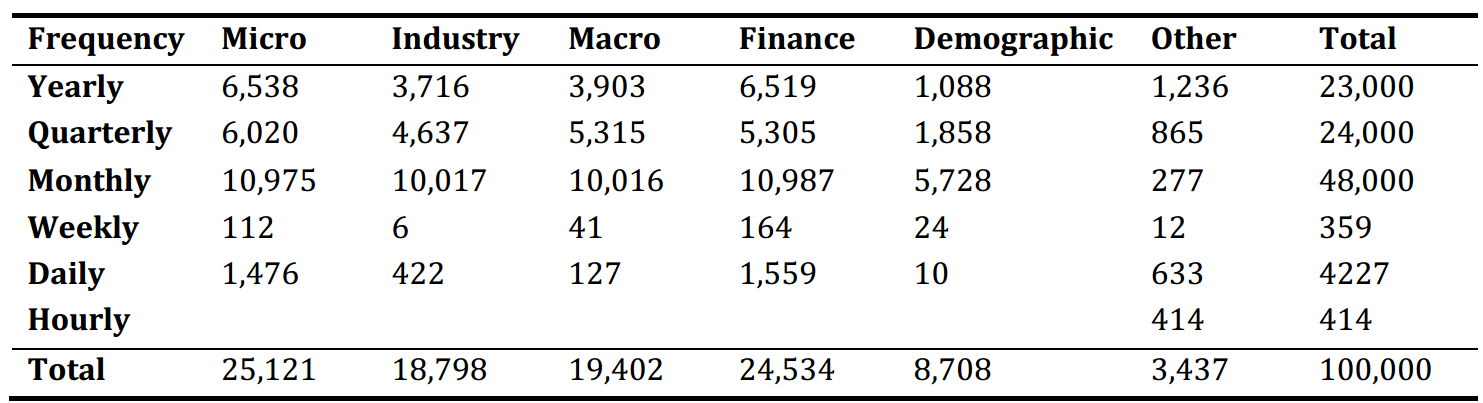
\includegraphics[scale=.58]{../images/M4_data_overview.png} 
\caption{M4 data by domains and frequencies.}
\end{table}
They were chosen from a database of more than 900,000 time series. Each series consists of a date and a respective observation for that date, where the frequency determines the time between two observations. In this dataset, all frequencies are equidistant which means that the time between two observations is constant.  Common characteristics of time series include seasonal patterns, cyclic behavior, as well as trends that the model has to capture. Given the behavior of the series, the method has to extrapolate the series into the future. The number of future observations (forecast horizon) that had to be forecasted was given:
\begin{table}[h]
\label{tab_horizons}
\centering
\textbf{M4 Data - Forecast Horizons}\par\medskip
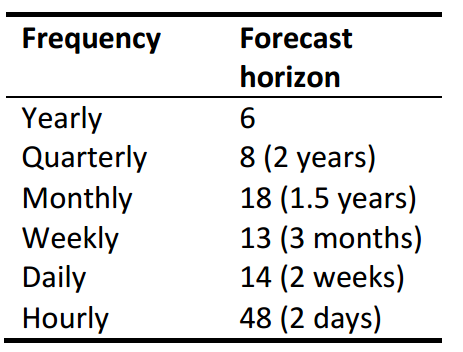
\includegraphics[scale=0.6]{../images/M4_data_forecast_horizon.png} 
\caption{Forecast horizons by frequency of the data.}
\end{table}
A key challenge for the prediction method is the high diversity of the data. Some data exhibit cyclical behavior, whereas other series exhibit up-/ downward trends, or varying seasonal patterns. Capturing the behavior accurately for all series is the goal of time series forecasting. 

\subsection{Exploratory Visualization}
The dataset is highly diverse with respect to domain and frequency. For each series there exists a training set as well as extended test set. The test set consists of the train set and the additional, previously unknown observations to be forecasted. A randomly chosen example series from the hourly M4 dataset is depicted below: 
\begin{figure}[h]
\label{series338}
\centering
\textbf{M4 Hourly - Series \#338}\par\medskip
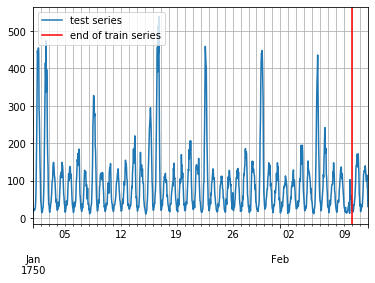
\includegraphics[scale=0.75]{../images/train_test_plot_m4_hourly338.png} 
\caption{Example series over time. The vertical red line indicates where the training data ends and the test data begins.}
\end{figure}

\subsection{Algorithms and Techniques}
The first of the three algorithms is the  \textbf{Deep Autoregressive Recurrent Neural Network (DeepAR)} method, introduced by Salinas et al. (2017). In the AWS Sageaker for ML in the cloud, it is the sole built-in time series prediction algorithm. DeepAR uses autoregressive features that are used as the inputs to a recurrent neural network. The RNN uses LSTM cells as default but can also be changed to GRU cells. Previous observations are utilized as inputs which makes this algorithm autoregressive. Autoregressive features are included based on the frequency of the data.

Rangapuram et al. (2018) introduced \textbf{Deep State Space Models (DeepState)}. DeepState combines state space models (SSM) with a recurrent neural network architecture that calculates the optimal parameters for the SSM. The SSM is applied locally to the individual time series. The parameters are determined by a RNN which is trained jointly on all available series. Hence, this algorithm combines a local with a global approach.

Furthermore, I included the \textbf{Deep Factor - RNN} by Wang et al. (2019). This hybrid algorithm uses any local method specific to each time series in the dataset as well as a global RNN trained on the entire data. For now, the only local method that is available is another RNN. Hence, the model combines a local RNN with a global RNN (\textbf{DF-RNN} in the following). Main differences between the algorithms: 
\begin{itemize}
\item \textbf{DeepAR} - Pure RNN that uses autoregressive features as inputs. 
\item \textbf{DeepState} - Uses global RNN to determine the best parameters of the local SSM.
\item \textbf{DF-RNN} - Hybrid of a local method (here: RNN) applied to individual time series that is combined with a global RNN that is trained jointly on all time series.
\end{itemize}
The training process for all three algorithms uses a fixed window approach. During training, batches of time series windows in the training data are fed to the algorithm. Each time series window is a sliced version of the entire series starting at different points of the series and has length of the training range plus prediction range. Here, the prediction range corresponds to the forecasting horizon of our model. Stochastic Gradient Descent (SGD) is used and during the training process the epoch with the smallest loss is chosen for the final model.


\subsection{Benchmarks}
In addition to providing a rich dataset across frequencies and domains, a key contribution of the M4 competition is the provision of a rich set of benchmark methods. Not only the metrics of the competition winners but also results for commonly used methods, in particular ARIMA and ES, are provided in Hyndman et al. (2019). In the discussion of the results I will focus on the relative performance of the RNN-based methods with respect to: 
\begin{enumerate}
\item Seasonally adjusted naive predictions (Naive2)
\item Traditional methods (ARIMA and ES) and combination benchmark (Comb)
\item Overall winning method of Smyl (2019), runner-up by Montero-Manso et al. (2019) as well as the winning method of the frequency under consideration.
\end{enumerate}

\section{Methodology}
\subsection{Data Preprocesing}
The data has to be prepared to be a valid input to the algorithms. Inputs are required to be in a \textbf{JSON Lines}-like format which in python is essentially a dictionary of dictionaries (nested dictionary). Inputs must contain at least the following keys with their respective content: 
\begin{itemize}
\item \texttt{`start`} - Timestamp with the format YYYY-MM-DD HH:MM:SS and the respective frequency of the data
\item \texttt{`target`} - An array of floats or integers that represents the target series of interest. 
\end{itemize}
An example input file takes the form
\begin{lstlisting}[frame=single]
# get first entry in dataset.train
entry = list(dataset.train)[0]

# first entry
entry
>>> {'start': Timestamp('1750-01-01 00:00:00', freq='H'),
 'target': array([605., 586., 586., ..., 521.], dtype=float32)
\end{lstlisting}
Additional keys are optional but often helpful in improving forecast accuracy. Here, the M4 competition does not provide additional covariates to the data.

\subsection{Implementation}
% Process for which metrics, algorithms, and techniques were implemented with the given datasets or input data has been thoroughly documented. Complications that occured during the coding process are discussed.
To obtain the results of the paper I used the \textbf{gluonts} library that is built on the deep learning library \textbf{MXNet}. For all three algorithms I proceeded in a similar way. 

First, I implemented a function that takes in the following arguments: 

\begin{itemize}
\item data - name of the built-in data in gluonts that was used 
\item seed - a seed that fixes the random numbers. Using the same seed results can be reproduced.
\item epochs - Number of epochs a model is trained
\item batches - Number of batches per epoch that are used. Each epoch the algorithm is fed using this many training examples.
\end{itemize}
\begin{lstlisting}[frame=single]
def deepar(data="m4_weekly", seed=42, epochs=100, batches=50):
    
    dataset = get_dataset(data, regenerate=False)
    mx.random.seed(seed)
    np.random.seed(seed)
    ...
\end{lstlisting}
Applying this function on a dataset yields results aforementioned accuracy measures: 
\begin{lstlisting}[frame=single]
res = deepar(data="m4_weekly", seed=42, epochs=1, batches=50)
pprint(res)

>>> {'MASE': 5.54378962,
 'MSIS': 54.72282354,
 'epochs': 1,
 'sMAPE': 0.12889508,
 'seed': 42,
 'wQuantileLoss[0.5]': 0.09491686,
 'wQuantileLoss[0.9]': 0.07740071}
\end{lstlisting}
A key finding was the instability of the algorithms. Applying the same algrithm with the same hyperparameters (i.e. epochs and batches) on one identical dataset leads to completely different results due to variability in the random numbers that are used. Hence, I had to implement a way to make the results reproducible by including seeds.

Also, in order to cancel out some of the variation in the results between iterations, I needed to repeat the experiments several times. For this, I wrote a loop that applies the respective function over a range of seeds and repeated the experiments holding the epochs and number of batches constant. The results show the median of three trials.

\begin{lstlisting}[frame=single]
results = []

data="m4_monthly"
epochs=100
batches=50

if __name__ == "__main__":
    for i in range(42, 45):
        print("Seed:", i)
        res = deepar(data, seed=i, epochs, batches)
        pprint(res)
        results.append(res)
\end{lstlisting}
This experimental arrangement ensures that the results are reproducible and meaningful by using seeds and several trials.

\subsection{Refinement}
A problem for an efficient implentation of the algorithms is the diverse nature of the data and the many different options of hyperparameters. 
%Difference in data 
The number of series within the four datasets range from 359 (M4 weekly) to 48,000 series (M4 monthly). Moreover, the data stems from different domains. There is seemingly no relation between the data. Aforementioned cross-learning by exploiting common patterns and dependencies seems difficult in this setting.
%Hyperparameter
Also, these algorithms allow many arguments to be determined such as prediction length of the forecasting horizon, context length to consider, number of RNN layers, number of RNN cells for each layer, or dropout rate just to mention a few of them. Besides prediction length which is fixed due to the restrictions of the competiton, there are many flexible parts for each forecasting problem to be considered. 

A common solution to this problem is to employ hyperparameter optimization (HPO) techniques, such as grid search or random search. These HPO techniques bascially run different variations of the same algorithm to determine the best hyperparameters. This is not a viable option here. Some the models run for many hours per trial and running different variations multiplies computational costs. Due to limited resources I decided to start with the default values which should already deliver reasonable results and only adjusting the number of epochs, number of batches per epoch, and the seed of the random numbers.

\section{Results}
This section describes the results per frequency, starting from the lowest (hourly) to the highest one (monthly). For every combination of algorithm, data, epochs, and batches, only the median result of three trials is included in the table. Trials start with seed 42 because it is "the ultimate answer to life, the universe, and everything..." (Adams, 2005). 
Note that DeepState models are computationally more expensive. Hence, I limited experimentation with DeepState to an acceptable minimum as some models took more than 13 hours of CPU time per trial. Because this algorithm is more stable than the others it  shouldn't alter the conclusions on its accuracy.

\subsection{Model Evaluation and Validation}

\subsubsection*{M4 Hourly}
The hourly subset of the M4 data contains 414 time series. Given forecast horizon (i.e. the number of future observations) was 48, which corresponds to two days. 

\begin{table}[h]
\label{m4_hourly_results}
\centering
\textbf{M4 Hourly - Results}\par\medskip
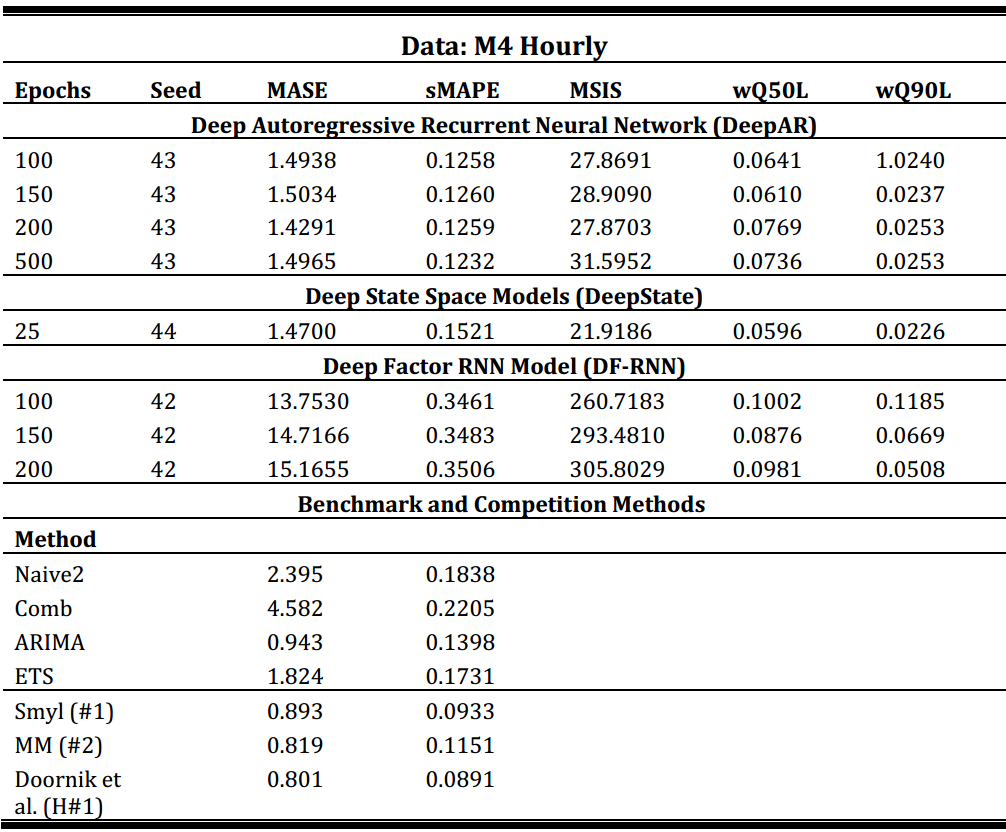
\includegraphics[scale=0.85]{../images/M4_hourly_results.png} 
\caption{Results for hourly M4 data.}
\end{table}

Table \ref{m4_hourly_results} illustrates the performance of aforementioned algorithms, respective benchmarks, and winning methods applied on the hourly data of the M4 data. 

It seems that DF-RNN is not able to capture hourly data at all. Comparing either its MASE or sMAPE to the seasonally adjusted naive forecast (Naive2) shows how bad it works. Note that the performance is even worse than a naive forecast that simply takes the previous value as forecast (value not shown in the table). 

With respect to Naive2 and the combination benchmark both models of DeepAR and DeepState show a higher accuracy. Moreover, they are also able to perform more accurate than ETS. However, the traditional ARIMA method that is based on modeling the autoregressive behavior of time series, outperforms both models with ease. 

Additionally, neither of the considered three algorithms comes close to the overall winning method by Smyl which is also based on recurrent neural networks. In addition, Montero-Manso (2019) and the best hourly method of Doornik et al. capture hourly data more precisely than the winning method. 

DeepAR and DeepState perform similarly in this setting. Their performance however is definitely not impressive. Note that this is a rather small dataset and model converge rather quick during training. 

\subsubsection*{M4 Daily}
Next, I will present the results for the M4 daily dataset which consists of 4227 series. The task is to predict the next 14 observations, i.e. 2 weeks. 

\begin{table}[h]
\label{m4_daily_results}
\centering
\textbf{M4 Daily - Results}\par\medskip
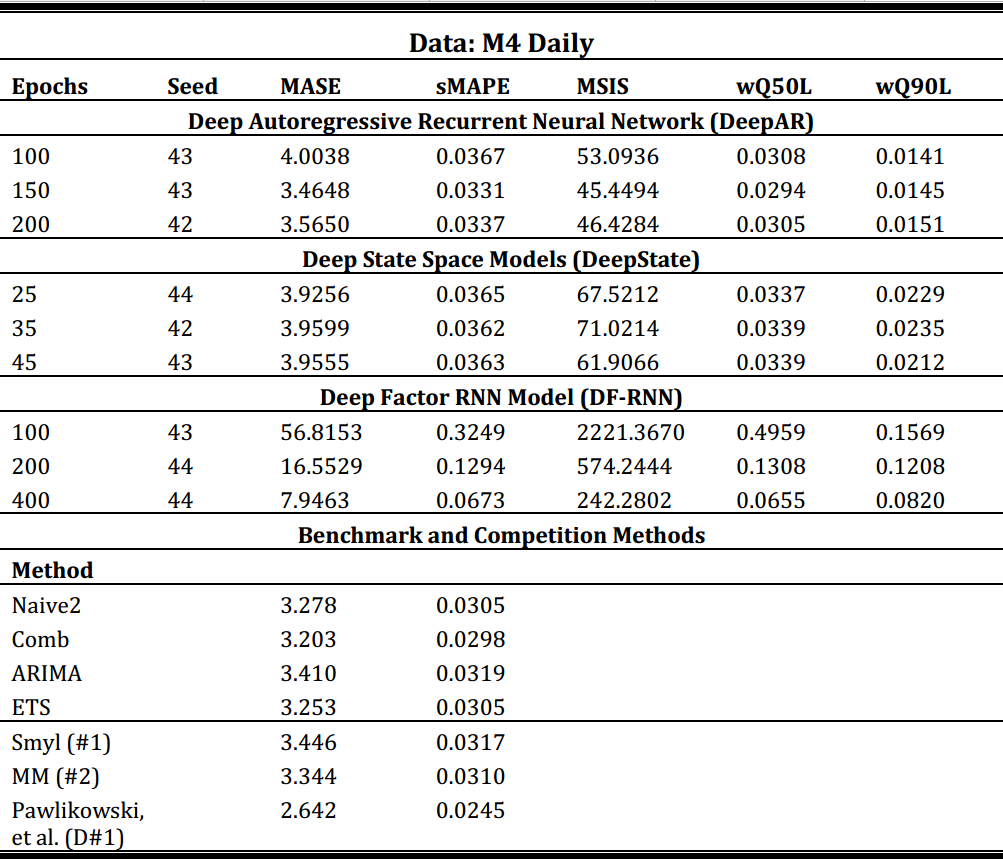
\includegraphics[scale=0.85]{../images/M4_daily_results.png} 
\caption{Results for M4 Daily data.}
\end{table}



\subsubsection*{M4 Weekly}
Among the M4 subsets by frequency, the M4 weekly dataset has the fewest with 359 individual series. Forecast range is 13 which is roughly equivalent to three months or one quarter. 

\begin{table}[h]
\label{m4_weekly_results}
\centering
\textbf{M4 Weekly - Results}\par\medskip
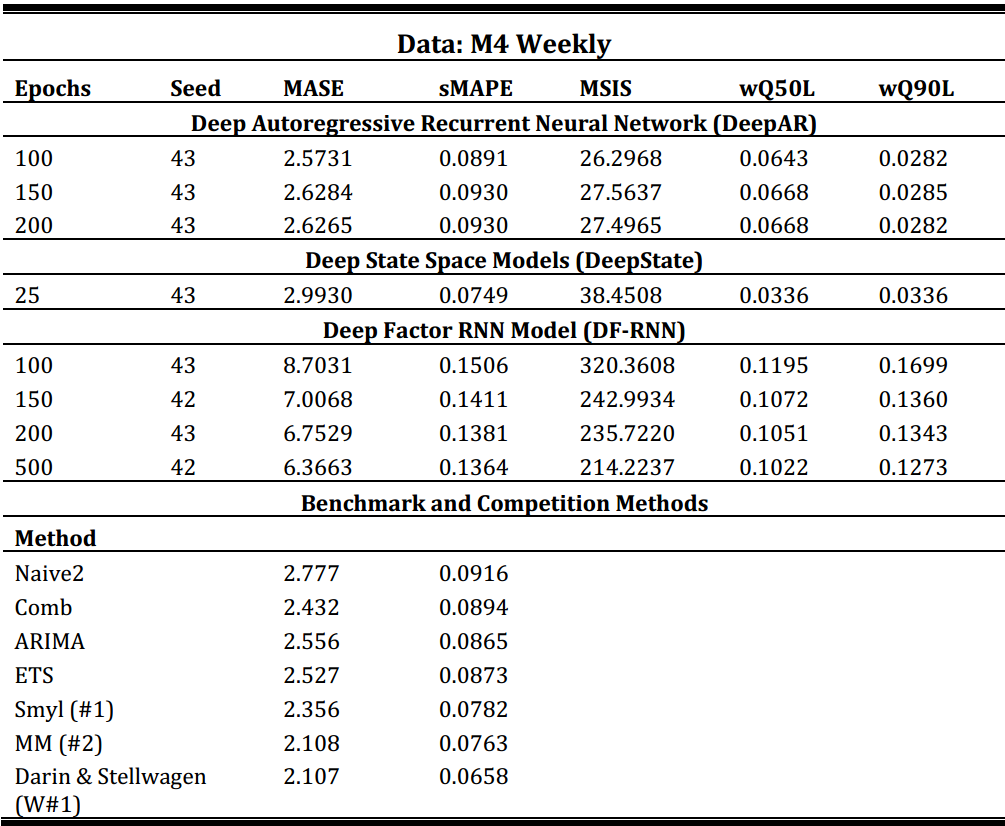
\includegraphics[scale=0.85]{../images/M4_weekly_results.png} 
\caption{Results for weekly M4 data.}
\end{table}

\subsubsection*{M4 Monthly}
The monthly data of the M4 competition contains 48,000 time series and is the largest among all frequencies. 

%Convergency issues


\begin{table}[h]
\label{m4_weekly_results}
\centering
\textbf{M4 Monthly - Results}\par\medskip
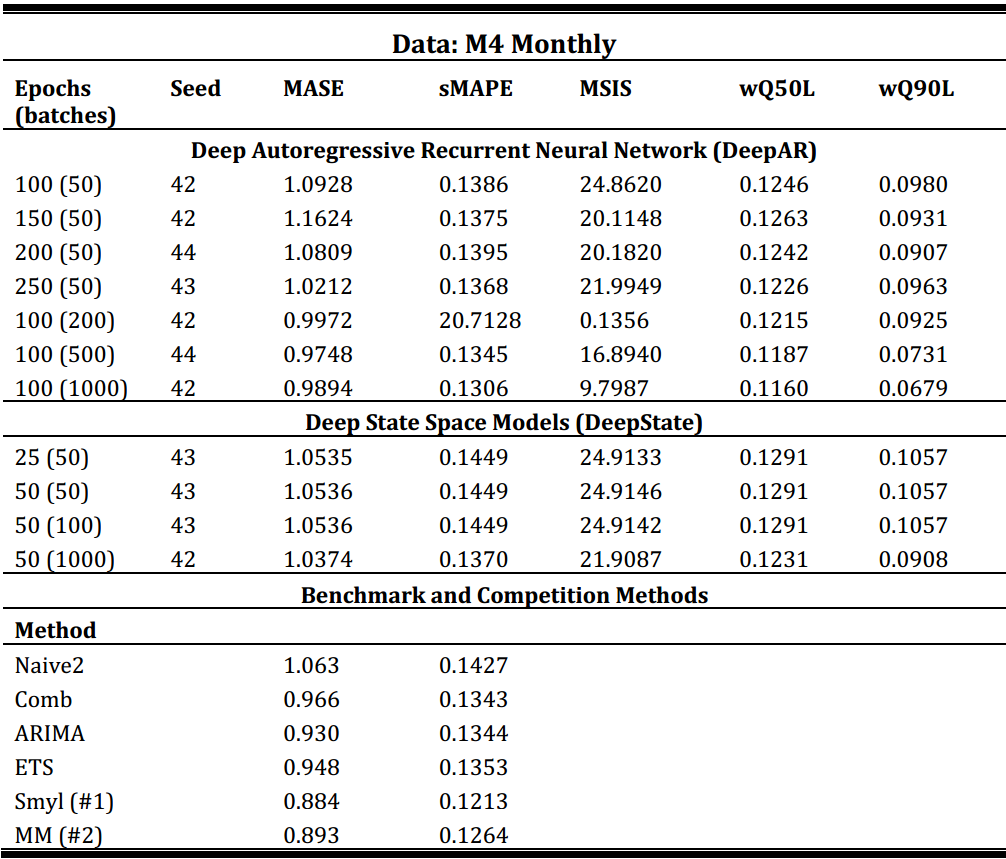
\includegraphics[scale=0.85]{../images/M4_monthly_results.png} 
\caption{Results for monthly M4 data.}
\end{table}

\subsection{Justification}
The main question of this project is to whether RNN-based algorithms may be a valuable tool in time series forecasting. 

%Conclusion (0.5-1 page)

%%%%%%%%%%%%%%%%%%%%%%%%%%%%%%%%%%%%%%%%%%%%%%%%%%%%%%%%%%%%%%%%%%%%%%%%%%%%%%%%%%%%%%%%%%%%%%%%%%%
%%%%%%%%%%%%%%%%%%%%%%%%%%%%%%%%%%%%%%%%%%%%%%%%%%%%%%%%%%%%%%%%%%%%%%%%%%%%%%%%%%%%%%%%%%%%%%%%%%%


%%%%%%%%%%%%%%%%%%%%%%%%%%%%%%%%%%%%%%%%%%%%%%%%%%%%%%%%%%%%%%%%%%%%%%%%%%%%%%%%%%%%%%%%%%%%%%%%%%%
%%%%%%%%%%%%%%%%%%%%%%%%%%%%%%%%%%%%%%%%%%%%%%%%%%%%%%%%%%%%%%%%%%%%%%%%%%%%%%%%%%%%%%%%%%%%%%%%%%%


%%%%%%%%%%%%%%%%%%%%%%%%%%%%%%%%%%%%%%%%%%%%%%%%%%%%%%%%%%%%%%%%%%%%%%%
%% Anhang %%%%%%%%%%%%%%%%%%%%%%%%%%%%%%%%%%%%%%%%%%%%%%%%%%%%%%%%%%%%%%
%%%%%%%%%%%%%%%%%%%%%%%%%%%%%%%%%%%%%%%%%%%%%%%%%%%%%%%%%%%%%%%%%%%%%%%
%% LITERATURE %%%%%%%%%%%%%%%%%%%%%%%%%%%%%%%%%%%%%%%%%%%%%%%%%%%%%%%%%%%%%

% View complete list of literature in database
%\nocite*

% List of references
\newpage
%\bibliography{dateiname.bib}
\bibliographystyle{plain}
 \begin{thebibliography}{------}
%alphabetisch sortieren

	\bibitem{Adams2005}
Adams, Douglas. "The Hitchhiker's Guide to the Galaxy". Del Rey Books. 2005

	\bibitem{Hyndman2019}
Hyndman, Rob J. "A brief history of forecasting competitions." \textit{International Journal of Forecasting (2019)}.
	
	\bibitem{HK2006}
Hyndman, Rob J., and Anne B. Koehler. "Another look at measures of forecast accuracy." \textit{International journal of forecasting 22.4 (2006): 679-688.}

	\bibitem{MEV2018}
Makridakis, Spyros, Evangelos Spiliotis, and Vassilios Assimakopoulos. "Statistical and Machine Learning forecasting methods: Concerns and ways forward." \textit{PloS one 13.3 (2018):
e0194889.}

	\bibitem{MEV2019}
Makridakis, Spyros, Evangelos Spiliotis, and Vassilios Assimakopoulos. "The M4 competition: 100,000 time series and 61 forecasting methods." \textit{International Journal of Forecasting
(2019).}

	\bibitem{MM2019}
Montero-Manso, Pablo, et al. "FFORMA: Feature-based forecast model averaging." \textit{International Journal of Forecasting (2019).}

	\bibitem{RSG+2018}
Rangapuram, Syama Sundar, et al. "Deep state space models for time series forecasting." \textit{Advances in Neural Information Processing Systems}. 2018.

	\bibitem{SFG2017}
Salinas, David, Valentin Flunkert, and Jan Gasthaus. "DeepAR: Probabilistic forecasting with autoregressive recurrent networks." \textit{arXiv preprint arXiv:1704.04110 (2017).}

	\bibitem{Smyl2019}
Smyl, Slawek. "A hybrid method of exponential smoothing and recurrent neural networks for time series forecasting." \textit{International Journal of Forecasting (2019).}

	\bibitem{SE+2019}
Spiliotis, Evangelos, et al. "Are forecasting competitions data representative of the reality?." \textit{International Journal of Forecasting (2019).}

	\bibitem{W+2019}
Wang, Yuyang, et al. "Deep Factors for Forecasting." \textit{arXiv preprint arXiv:1905.12417 (2019).}

 \end{thebibliography}


%%%%%%%%%%%%%%%%%%%%%%%%%%%%%%%%%%%%%%%%%%%%%%%%%%%%%%%%%%%%%%%%%%%%%%%
%% EIDESSTATTLICHE ERKL�RUNG  %%%%%%%%%%%%%%%%%%%%%%%%%%%%%%%%%%%%%%%%%
%\newpage
%\selectlanguage{ngerman}
%\section*{Eidesstattliche Erkl�rung}
%Hiermit versichere ich, dass ich die vorliegende Arbeit selbstst�ndig und ohne die Benutzung anderer als der angegebenen Hilfsmittel angefertigt habe. Alle Stellen, die w�rtlich oder sinngem�� aus ver�ffentlichten und nicht ver�ffentlichten Schriften entnommen wurden, sind als solche kenntlich gemacht.\\
%\\
%K�ln, den \today
%\\
%Unterschrift
%\selectlanguage{english}
\end{document}
